\documentclass[12pt,letterpaper, onecolumn]{exam}
\usepackage{amsmath}
\usepackage{amssymb}
\usepackage{graphicx}
\usepackage[lmargin=71pt, tmargin=1.2in]{geometry}  %For centering solution box

% \chead{\hline} % Un-comment to draw line below header
\thispagestyle{empty}   %For removing header/footer from page 1

\begin{document}

\begingroup  
    \centering
    \LARGE STATS 212\\
    \LARGE Homework#3 \\
    \large \today\\[0.5em]
    \large Samuel Molero\par
    \large samueljosemolero@tamu.edu\par
    \large Section: 501\par
\endgroup
\rule{\textwidth}{0.4pt}
\pointsdroppedatright   %Self-explanatory
\printanswers
\renewcommand{\solutiontitle}{\noindent\textbf{Ans:}\enspace}   %Replace "Ans:" with starting keyword in solution box

\begin{questions}

    \question Q1?
    \begin{solution}
        \begin{parts}
        \part 
        \begin{verbatim}
            df <- read.csv("Baseball-Salary-Data.csv")
            head(df)
            m1 <- lm(salary ~ . - player, data = df)
            summary(m1)
        \end{verbatim}
        Running the above code output the following results:\\
        \includegraphics[width=0.7\textwidth]{Homeworks/}
        \part The R square of 0.7014, which translates to 70.14\%\
        \part The coefficient for the predictor is -2.698 which predicts a decrease in salaries holding all the other variables constant.This could be due to the variation in salary data is explained by other variables such as home run and stolen bases.
        \part 
        \end{parts}
            
    \end{solution}
    
    \question Q2?
    \begin{solution}
        \begin{parts}
            \part 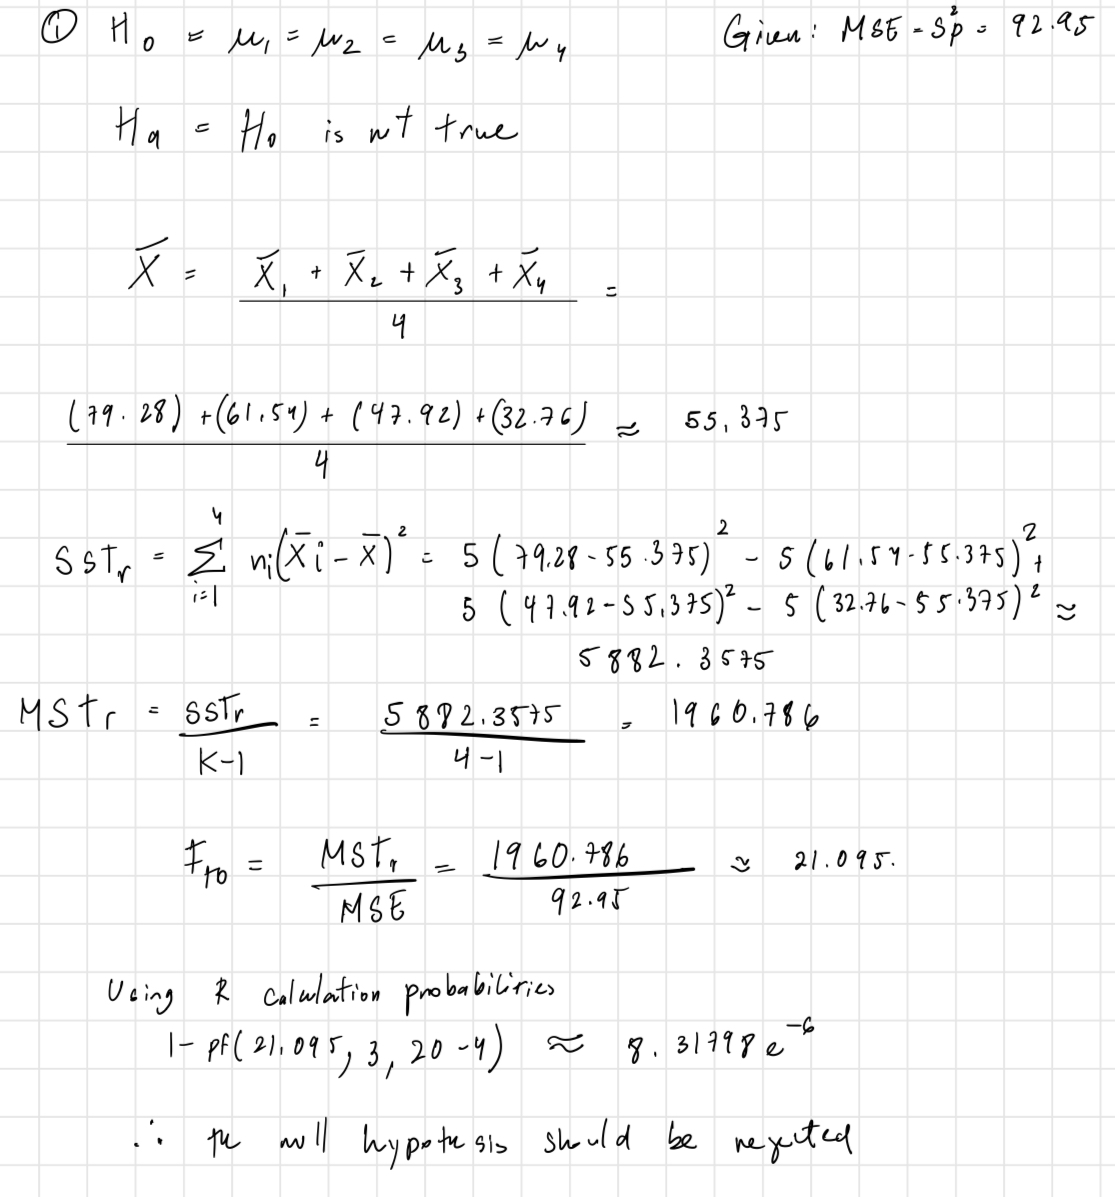
\includegraphics[width=0.7\textwidth]{Homeworks/partAHW3.jpg}
            \part
            \begin{verbatim} 
    dta2 <- read.table("SleepRem.txt", header = TRUE, sep = "")
    attach(dta2)
    fit <- aov(values ~ as.factor(ind), data = dta2)
    anova(fit)
    \end{verbatim}
    Using the above code snippet we get the following result:
    \begin{verbatim}
Response: values
        Df  Sum Sq  Mean Sq  F value  Pr(>F)    
find     3  5881.7 1960.58  21.093 8.322e-06 
Residuals 16 1487.1   92.95                      
    \end{verbatim}
    Given that is confirmed that the p-value is $8.322e-06$ the null hypothesis should be rejected.
    \part 
    \begin{verbatim}
      #To test variance
      anova(aov(resid(aov(values ~ ind))**2 ~ ind))
    \end{verbatim}
    Given that the p-value is 0.621. This suggests that the assumption of equal
    variance is approximately valid.
    \begin{verbatim}
    #to test stability
    shapiro.test(resid(aov(values ~ ind)))
    \end{verbatim}
     p-value = 0.1285 suggests that the normality assumption
    approximately holds.
    \end{parts}
    \begin{verbatim}
        fit = aov(values ~ find)
        boxplot(resid(fit))
        plot(fit, which=2)
        \end{verbatim}
       The Code snippets creates the following graphs:\\
    \center
    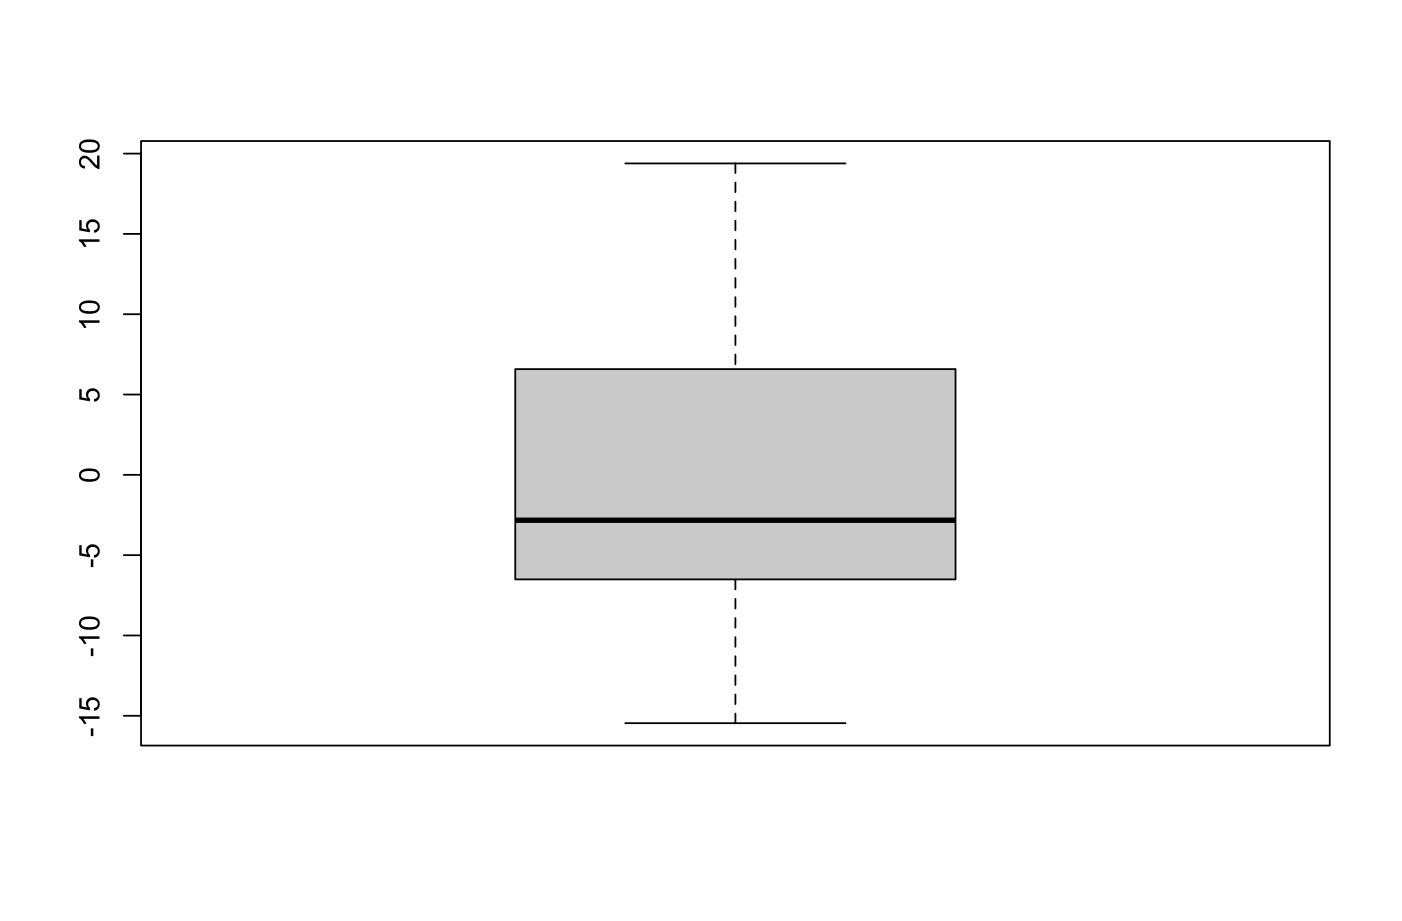
\includegraphics[width=0.7\textwidth]{Homeworks/Graph1HW3.png}\\
    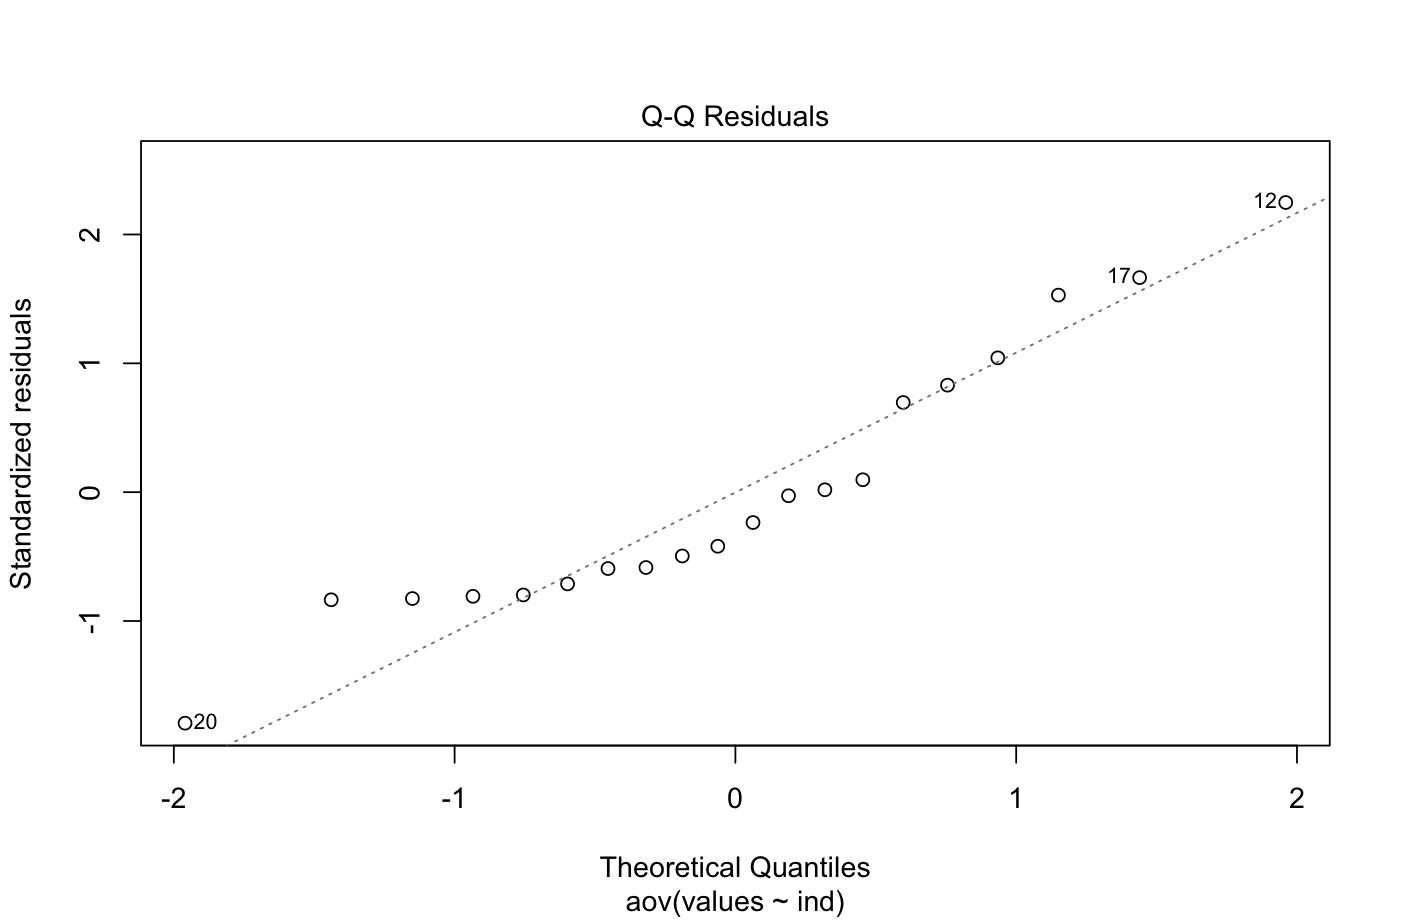
\includegraphics[width=0.7\textwidth]{Homeworks/Graph2HW3.png}\\
    plots also suggest that the normality assumption is approximately satisfied, in agreement with the Shapiro-Wilk test p-value.
    \end{solution}

    \pagebreak %Not necessary
    
    
\end{questions}
\end{document}